\documentclass[../main.tex]{subfiles}

\begin{document}

\chapter{Об’єктно-орієнтоване проектування ІС}

Якщо аналіз об’єкта проектування – це розробка відповідної логічної моделі, яка описує усі можливі та прийнятні варіанти розв’язання задач, які вказують, що повинна робити система, то проектування – це вироблення рішення відповідно до моделі аналізу, яке оптимізує набір критеріїв проектування, які  показують, як ця поведінка (робота) системи може бути реалізована \cite{diploma_guidelines}.
Оскільки, у даній роботі застосовується об’єктно-\linebreak[0]орієнтована технологія проектування, то проектна частина повинна складатися із таких етапів:

\begin{enumerate}
	\item Архітектурне проектування – описує логічну структуру інформаційної системи (програмні класи, підсистеми,  пакети) та їх зв’язки.
	\item Детальне проектування – описує структури даних та алгоритми всередині окремих класів. 
\end{enumerate}

\section{Архітектурне проектування}
Формування архітектури – перший і основний крок у розв’язанні завдання проектування, що закладає фундамент уявлення програмної системи, здатної виконувати весь спектр детальних вимог. \cite{diploma_guidelines2}

Створення архітектури – це проектування на найвищому рівні (логічна архітектура). Логічна архітектура описує систему в термінах її принципової організації у вигляді пакетів, програмних класів і підсистем. Вона називається логічною, оскільки не визначає способи розгортання цих елементів у різних операційних системах або на фізичних комп’ютерах в мережі (це відноситься до архітектури розгортання)~\cite{diploma_guidelines}.

Система Android надає різнобічну платформу додатків, на основі якої можна створювати інноваційні програми та ігри для мобільних пристроїв в середовищі мови Java. Важливо знати наступні основні концепції, що стосуються платформи додатків Android.

\subparagraph{Додатки мають кілька точок входу.}
Додатки для Android будуються з окремих компонентів, які можна викликати незалежно один від одного. Наприклад, окрема активність надає один екран для користувацького інтерфейсу, а служба незалежно виконує роботу у фоновому режимі.
	
За допомогою об'єкта Intent з одного компонента можна запустити інший. Також можна запустити компонент з іншої програми, наприклад, активність з картографічного додатка, щоб показати адресу. Ця модель формує кілька точок входу для однієї програми, і при цьому користувач може вибрати будь-який додаток за замовчуванням для виконання тієї чи іншої дії, яка може викликати інші додатки.
	
\subparagraph{Додатки адаптуються до різних пристроїв.}
Android надає адаптивну платформу додатків, яка дозволяє забезпечувати унікальні ресурси для різних конфігурацій пристроїв. Наприклад, можна створити різні файли XML макета для екранів різних розмірів, а система буде визначати, який макет використовувати, з урахуванням розміру екрану даного пристрою.

Якщо якимось функціям програми потрібне певне обладнання, наприклад камера, можна запитувати його наявність в пристрої під час виконання. При необхідності також можна оголошувати функції, які потрібні додатку, для того, щоб такі магазини додатків, як Google Play, не~дозволяли встановлювати додатки на пристроях, в яких цих функцій немає~\cite{android_4}.

\subsection{Компоненти Android-додатку}

Компоненти програми є частинками, з яких складається додаток для Android. Кожен компонент являє собою окрему точку, через яку система може увійти в додаток. Не всі компоненти є точками входу для користувача, а деякі з них залежать один від одного. При цьому кожен компонент є самостійною структурною одиницею і відіграє певну роль -- кожен з них являє собою унікальний елемент структури, який визначає роботу програми в цілому.

Компоненти програми можна віднести до одного з чотирьох типів. Компоненти кожного типу призначені для певної мети, вони мають власний життєвий цикл, який визначає спосіб створення і припинення існування компонента.

\subparagraph{Активності.}
Активність (Activity) являє собою один екран з користувацьким інтерфейсом. Наприклад, в додатку для роботи з електронною поштою одна активність може служити для відображення списку нових повідомлень, інша -- для створення повідомлення і третя -- для читання повідомлень. Попри те, що активності спільно формують чітку взаємодію користувача з додатком по роботі з електронною поштою, кожна з них не залежить від інших. Будь-які з цих активностей можуть бути запущені іншим додатком (якщо додаток дозволяє це). Наприклад, додаток для камери може запустити активність в додатку по роботі з електронною поштою, яка створює нове повідомлення, щоб користувач міг відіслати фотографію.

\subparagraph{Служби.}
Служба (Service) являє собою компонент, який працює у фоновому режимі й виконує тривалі операції, пов'язані з роботою віддалених процесів. Служба не має користувацького інтерфейсу. Наприклад, вона може відтворювати музику у фоновому режимі, поки користувач працює в іншому додатку, або може отримувати дані через мережу, не блокуючи взаємодію користувача з активністю. Служба може бути запущена іншим компонентом, який потім буде взаємодіяти з нею.

\subparagraph{Постачальники контенту.}
Постачальник контенту (Content provider) управляє загальним набором даних програми. Дані можна зберігати в файловій системі, базі даних, інтернеті або будь-якому іншому постійному місці зберігання, до якого у додатка є доступ. За допомогою постачальника контенту інші додатки можуть запитувати або навіть змінювати дані (якщо постачальник контенту дозволяє робити це). Наприклад, в системі Android є постачальник контенту, який управляє інформацією контактів користувача. Будь-який додаток, що отримав відповідні дозволи, може запитати частину цього постачальника контенту, для читання і запису відомостей про певну людину.

\subparagraph{Приймачі широкомовних повідомлень.}
Приймач широкомовних повідомлень (Broadcast receiver) являє собою компонент, який реагує на оголошення поширювані по всій системі. Багато з цих оголошень розсилає система -- наприклад, оголошення про те, що екран вимкнувся, акумулятор розряджений або був зроблений фотознімок. Оголошення також можуть розсилатися додатками, наприклад, щоб повідомити іншу програму про те, що якісь дані були завантажені на пристрій і тепер готові для використання. Хоча приймачі широкомовних повідомлень не мають інтерфейсу користувача, вони можуть створювати повідомлення в рядку стану, щоб попередити користувача про подію. Однак, найчастіше вони є просто шлюзом для інших компонентів і призначені для виконання мінімального обсягу роботи. Наприклад, вони можуть ініціювати виконання службою певних дій при виникненні події.

Унікальною особливістю системи Android є те, що будь-який додаток може запустити компонент іншого додатку. Наприклад, якщо розробник хоче дати користувачеві можливість фотографувати, використовуючи камеру пристрою, то, якщо є інший додаток, який може виконати цю дію, замість того щоб розробити активність фотографування в своєму додатку, він може викликати такий додаток. Не потрібно впроваджувати код з програми для камери або навіть встановлювати на нього посилання. Замість цього можна просто запустити активність фотографування з програми для камери. По завершенні цієї активності фотографія буде повернута в додаток, і її можна буде використовувати. Для користувача це буде виглядати як один додаток.

Коли система запускає компонент, вона запускає процес для цього додатка (якщо він ще не був запущений) і створює екземпляри класів, які потрібні цьому компоненту. Наприклад, якщо додаток запустить активність фотографування в додатку для камери, ця активність буде виконуватися в процесі, який відноситься до цього стороннього додатку. Тому, на відміну від додатків для більшості інших систем, в додатках для Android відсутня єдина точка входу.

Оскільки система виконує кожен додаток в окремому процесі з правами доступу до файлів, які обмежують доступ до інших додатків, він не~може безпосередньо викликати компонент з іншого додатку. Це може зробити сама система Android. Тому, щоб викликати компонент в іншому додатку, необхідно повідомити системі про свій намір (Intent) запустити певний компонент. Після цього система активує його.

Для запуску компонента додатку системі Android необхідно знати, що компонент існує. Для цього вона читає файл маніфесту додатка (AndroidManifest.xml). У цьому файлі, який повинен знаходитися в кореневій теці програми, повинні бути оголошені всі компоненти програми.

Оскільки користувач здійснює різні переходи в додатку, екземпляри активностей в додатку проходять через різні стани їхнього життєвого циклу. Клас активності забезпечує ряд зворотних викликів, які дозволяють активності знати, що стан змінився: система створює, зупиняє чи відновлює активність, або знищує процес, в якому знаходиться активність.

У методах життєвого циклу, можна оголосити, як активність буде поводити себе, коли користувач залишить її, а потім здійснить повторний вхід. Наприклад, якщо створюється потоковий відеоплеєр, є можливість призупинити відео та зупинити з'єднання з мережею, коли користувач перемикається на іншу програму. Коли він повертається, можна відновити підключення та дозволити користувачеві відновити відтворення відео з того ж місця. Кожен метод життєвого циклу дозволяє виконувати роботу, яка потрібна при конкретному стані активності. Використання правильних станів для потрібних дій зробить додаток надійнішим та більш продуктивним. Наприклад, хороша реалізація методів життєвого циклу дозволить додатку уникнути:

\begin{enumerate}
	\item Збоїв при отриманні користувачем телефонного дзвінка або перемиканні на іншу програму.
	\item Споживання цінних системних ресурсів, у випадку, коли користувач активно не використовує його.
	\item Втрати прогресу користувача, якщо він залишить додаток і повернутися до нього пізніше.
	\item Збоїв чи втрати прогресу, якщо екран змінить свою орієнтацію на пейзажну чи портретну.
\end{enumerate}

Для навігації між етапами життєвого циклу активності, клас \textit{Activity} забезпечує основний набір з шести зворотних викликів. Детальна схема життєвого циклу активності зображена  на рис. \ref{diagram:activity_lifecycle}

\begin{figure}[H]
	\centering
	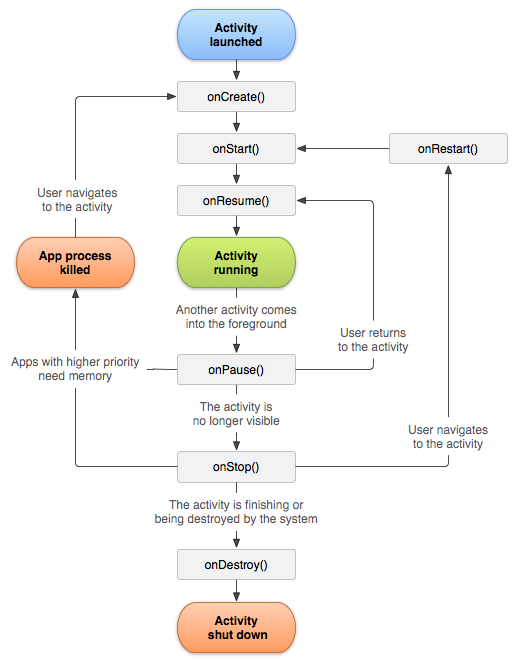
\includegraphics[width=0.8\textwidth]{activity_lifecycle}
	\caption{Життєвий цикл активності}
	\label{diagram:activity_lifecycle}
\end{figure}

\subsection{Побудова діаграми пакетів}
Одним з важливих етапів архітектурного проектування є побудова діаграми пакетів. Діаграма пакетів є діаграмою, яка містить пакети класів і залежності між ними. Вона описує архітектурну основу системи та допомагає в управлінні масштабами й складністю системи. 

Діаграма пакетів для додатка зображена на рис. \ref{diagram:packages}.
\vspace{\baselineskip}

\begin{figure}[H]
	\centering
	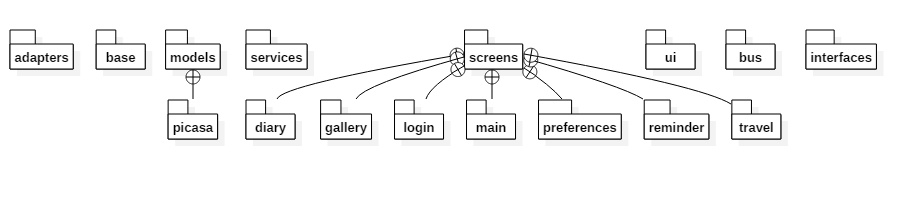
\includegraphics[width=1\textwidth]{diagram_packages}
	\caption{Діаграма пакетів для Android-щоденника}
	\label{diagram:packages}
\end{figure}

Пакет \textit{\textbf{adapters}} призначений для адаптерів. Адаптер -- це об'єкт, що діє як міст між представленням (view) і даними для цього представлення. Він забезпечує доступ до елементів даних. Також, адаптер відповідальний за подання представлення для кожного елемента в наборі даних \cite{adapter}. 

В пакеті \textit{\textbf{models}} будуть знаходитися класи моделей, що необхідні для взаємодії з базою даних чи іншими сервісами. Пакет \textit{\textbf{screens}} призначений для класів активностей, що являють собою окремі екрани додатку, тому в нього були додані додаткові пакети, щоб розділити екрани по областях, за які вони відповідають. Пакет \textit{\textbf{services}} буде містити служби, а пакети \textit{\textbf{ui}}, \textit{\textbf{bus}} та \textit{\textbf{interfaces}} -- компоненти, що відповідають за інтерфейс користувача, шину подій та Java інтерфейси відповідно. 

%TODO: move this to 3.2
\subsection{Побудова діаграми компонентів}
Ще одним будівельним блоком для створення архітектури об'єктно-\linebreak[0]орієнтованої системи вважається компонент. Діаграма компонентів показує розбиття програмної системи на структурні компоненти та залежності між компонентами. В якості фізичних компонентів можуть бути файли, бібліотеки, модулі, виконувані файли, пакети і т.п. У багатьох середовищах розробки модуль або компонент відповідає файлу. Стрілки, що з'єднують модулі, показують відносини взаємозалежності аналогічні тим, які мають місце при компіляції вихідних текстів програм. Основними графічними елементами діаграми компонентів є компоненти, інтерфейси й залежності між ними. 

Клас \textit{Application} є базовим класом для підтримки глобального стану програми. Для того, щоб надати йому власну реалізацію, потрібно створити підклас і вказати його повне ім'я в файлі маніфесту. В нашому випадку таким підкласом є \textit{App}. Він створюється в першу чергу, до того, як процес для додатка/пакета створиться.

Активності, яким потрібна однакова базова логіка, наслідуються від класу \textit{BaseActivity}. Всі сервіси додатку наслідуються від класу \textit{Service} або \textit{IntentService} та мають бути вказані в файлі маніфесту. Детальну структуру компонентів додатку зображено на рис. \ref{diagram:hierarchy} (стор.~\pageref{diagram:hierarchy}).

% \begin{figure}[H] % TODO думаю, тут все-таки краще спочатку пустити далі текст, далі розмістити рисунок. Дозволяє позбутися надто великих вертикальних дірок, вимогами розд.6.4 цілком допускається, і насправді активно використовується у практиці верстки взагалі.
\begin{figure}[p]
	\centering
	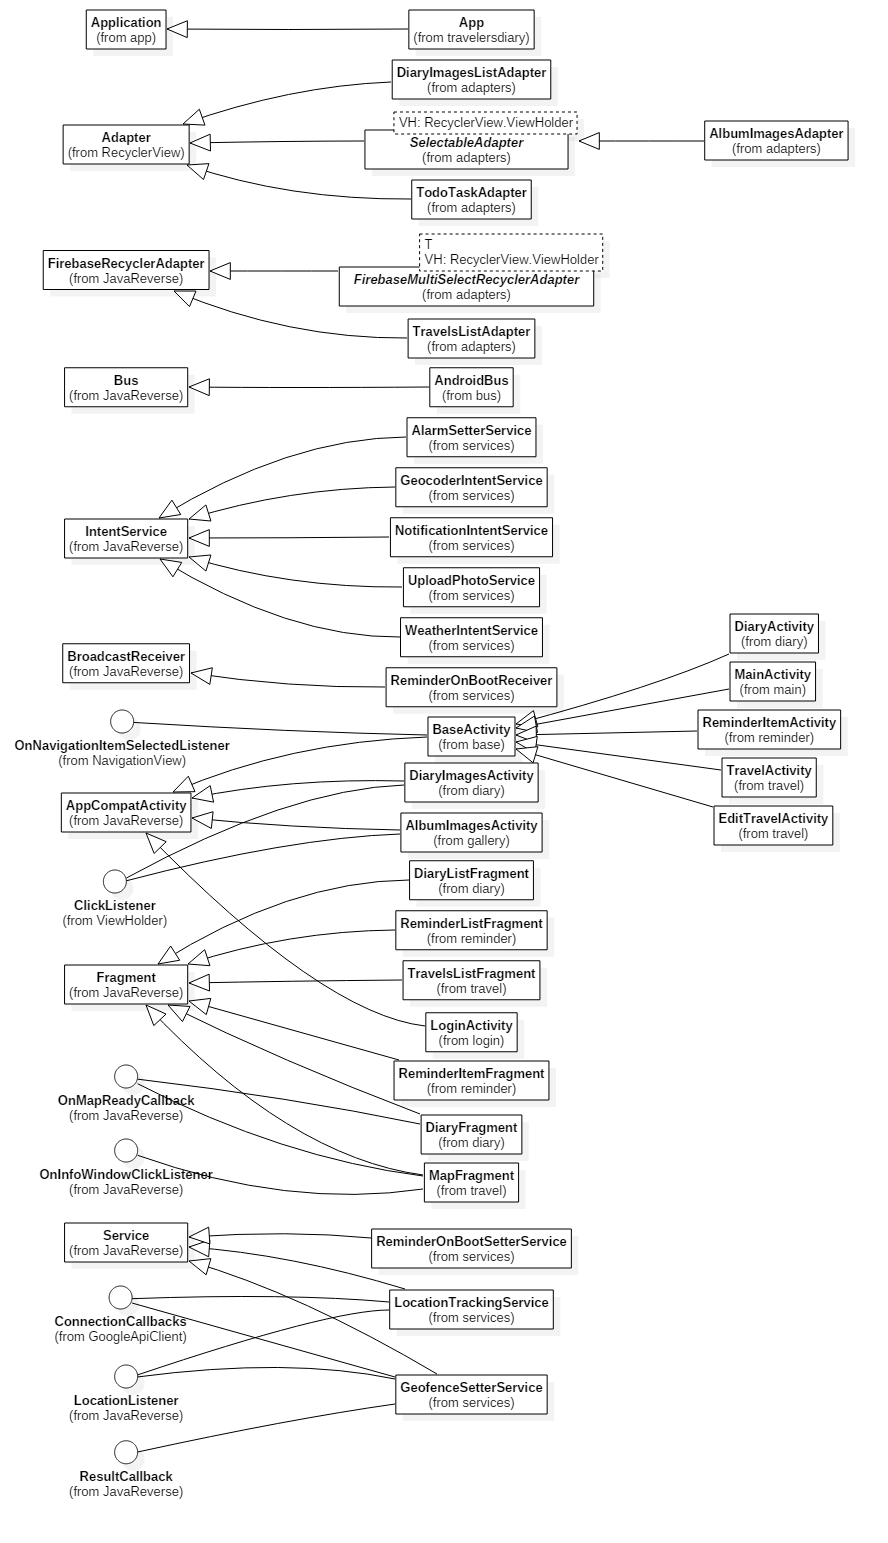
\includegraphics[height=0.8\textheight]{diagram_hierarchy}
	\caption{Діаграма компонентів Android-щоденника}
	\label{diagram:hierarchy}
\end{figure}

\section{Детальне проектування}

%TODO: move this to 4.1.2
Функціонально, додаток складається з наведених нижче модулів (активностей та фрагментів). Активність є схемою представлення Android-додатків. Кожен екран користувацькокого інтерфейсу представлений класом \textit{Activity} і по суті є окремою формою додатка. Android-додаток може складатися з декількох активностей і може перемикатися між ними під час виконання програми. 

Фрагмент (клас \textit{Fragment}) представляє поведінку або частину користувацького інтерфейсу в активностях. Можливе об'єднання кількох фрагментів в одній активності для побудови багатопанельного інтерфейсу та повторного використання фрагмента в декількох активностях. Фрагмент можна розглядати як модульну частину активності. Така частина має свій життєвий цикл і самостійно обробляє події введення. Крім того, її можна додати або видалити безпосередньо під час виконання активності. Це щось на зразок вкладеної активності, яку можна багаторазово використовувати в різних активностях.

При запуску додатку, користувач потрапляє на активність авторизації. Вона містить логотип, назву додатку та кнопку авторизації, пісня натиснення якої  користувачеві пропонується вибрати один з уже існуючих чи додати новий Google акаунт. Пісня успішної авторизації користувач потрапляє на головний екран додатку.

Головний екран містить бокове меню (\textit{Navigation Drawer}), яке містить три категорії: подорожі, щоденник та планувальник. При виборі категорії фрагмент, що знаходиться в цій активності, замінюється на той, що відповідає цій категорії. За замовчуванням обрана категорія \textit{подорожі}, тому головна активність містить фрагмент зі списком подорожей. При виборі категорії \textit{щоденник} чи \textit{планувальник}, цей фрагмент замінюється на фрагмент зі списком записів щоденника чи планувальника відповідно. При виборі елементу зі списку, відбувається перехід до відповідних активностей.

Активність подорожі відкривається при виборі подорожі зі списку. Вона містить сторінки на яких відображаються фрагмент зі списком записів щоденника, фрагмент зі списком записів планувальника та фрагмент з картою. З меню, що міститься в цій активності, можливий перехід до активності редагування подорожі.

Активність запису щоденника містить текст запису, список прикріплених фото та інформацію про погодні умови та місце створення запису. Для перегляду всіх прикріплених фото відкривається нова активність, що містить список цих фото. Також можливе редагування чи видалення запису. Активність запису планувальника слугує для його перегляду та редагування.

Фрагмент, що містить карту відображається на одній зі сторінок в активності подорожі. На цій карті зображується записаний трек переміщень та мітки, які можуть означати початок чи кінець треку та запис щоденника чи планувальника. Фрагменти зі списками подорожей, записів щоденника чи планувальника завантажують відповідну інформацію з бази даних та на підставі отриманих даних формують динамічний список об'єктів за допомогою адаптеру \textit{FirebaseRecyclerAdapter}.

Діаграма активностей та фрагментів розроблюваного додатка представлена на рис. \ref{diagram:activities}.

\begin{figure}[H]
	\centering
	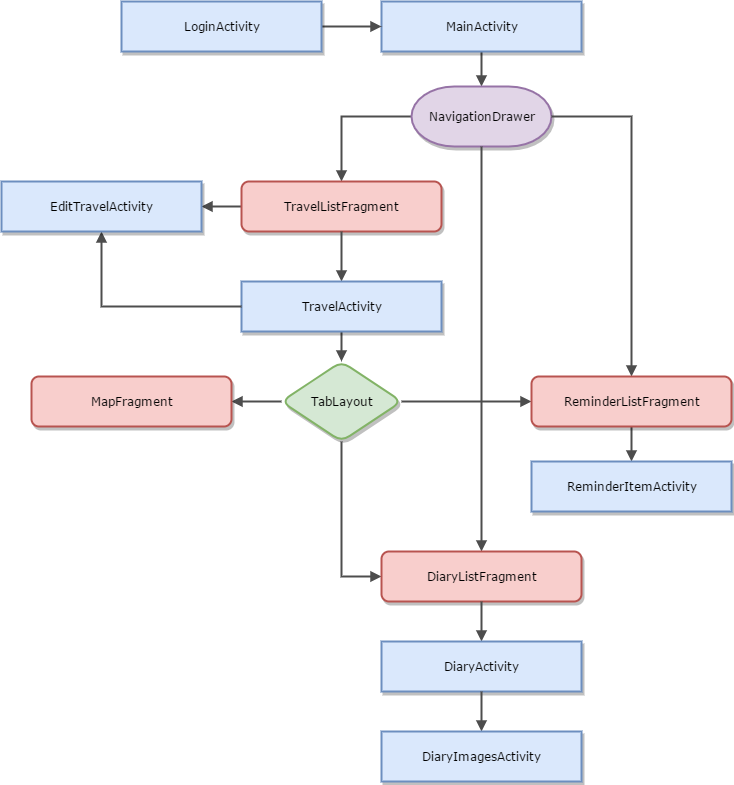
\includegraphics[width=0.6\textheight]{diagram_activities}
	\caption{Діаграма активностей та фрагментів}
	\label{diagram:activities}
\end{figure}

Для того, щоб додаток міг взаємодіяти з базою даних, зберігати та зчитувати дані, потрібно спроектувати моделі для необхідних об'єктів. Основними об'єктами є подорож, запис щоденника та планувальника.

Подорож повинна мати назву, опис, час створення, початку та завершення, а також індикатор, який вказує активна вона чи ні. Додатково містяться поля для обкладинки подорожі. У записі щоденника буде міститися назва, текст, список фото, а також час створення та інформація про погодні умови і місце створення запису. Запис планувальника також буде містити назву та текст, відмітку про виконання та відомості про нагадування, такі як час та дата чи місце нагадування.

Для збереження інформації про погоду було створено модель, яка містить поля для температури, тиску та інших погодних параметрів. Для збереження інформації про місцезнаходження для запису щоденника, було створено модель, що містить назву країни, міста, вулиці та інші відомості про це місце. Для запису треку переміщень необхідно зберігати координати користувача з деякою періодичністю. Для цього було створено модель, що містить мапу, ключем в якій є час, а значенням -- координати користувача.

Детальна діаграма моделей для додатка зображена на рис.~\ref{diagram:models} (стор.~\pageref{diagram:models}).

\begin{figure}[pt] % TODO див. позаминулий рисунок
% \begin{figure}[H]
	\centering
	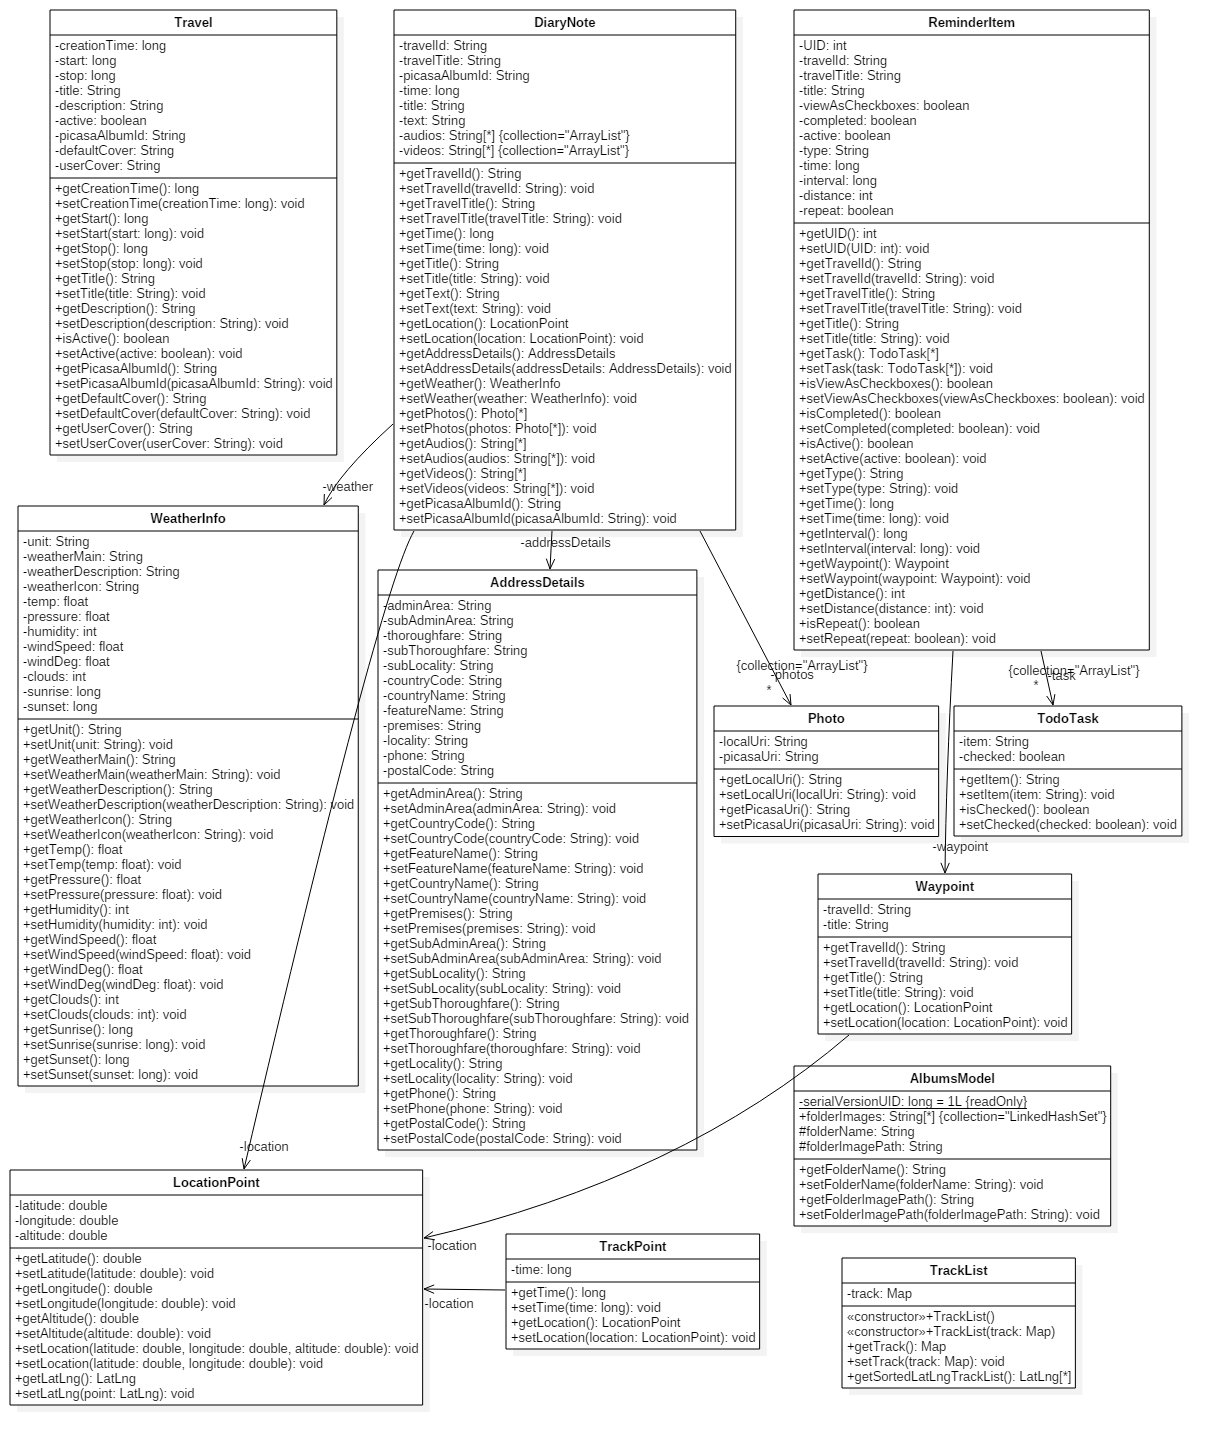
\includegraphics[height=0.73\textheight]{diagram_models}
	\caption{Діаграма моделей Android-щоденника}
	\label{diagram:models}
\end{figure}

\section{Розгортання програмної системи на апаратних засобах}

Оскільки при розробці викорисловувалися сервіси Firebase, система може бути розгорнута під будь-яку платформу, що підтримує Firebase (Web, iOS, Unity та ін.). За темою роботи проводилася розробка Android клієнту. Діаграму розгортання системи представлено на рис. \ref{diagram:deployment}.

Для функціонування додатку необхідна операційна система Android версії 4.2 (API 16) і вище.

\begin{figure}[H]
	\centering
	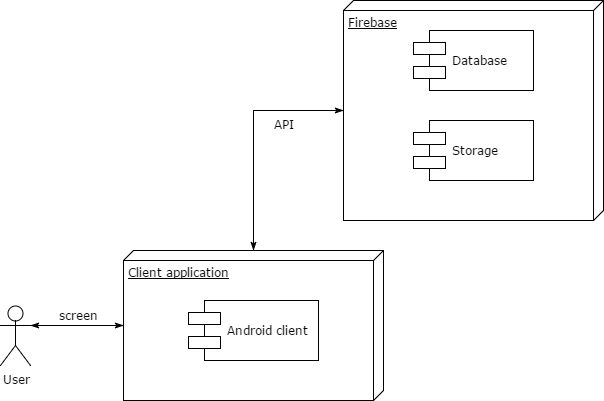
\includegraphics[width=0.8\textwidth]{diagram_deployment}
	\caption{Діаграма розгортання системи}
	\label{diagram:deployment}
\end{figure}

\section{Висновки}

%TODO: Висновки до розділу (не більш 1-2 сторінки). Розмір одного висновку приблизно – один абзац (5-7 рядків). Висновки цього розділу є важливою і значущою частиною роботи.

Результатом роботи над даним розділом є формування та створення архітектури, що є основними крокома у розв'занні завдання проектування. Вони закладають фундамент програмної системи, описують систему в термінах її принципової організації у вигляді пакетів, програмних класів і підсистем.

Також, було проаналізовано основні концепції платформи Android додатків, та розглянуто основні компоненти, з яких може складатися Android-додаток. Було побудовано діаграму пакетів, на якій відображено пакети та зв'язки між ними, та діаграму компонентів, яка показує розбиття програмної системи на структурні компоненти та залежності між ними.

%TODO Проведено детальне проектування системи

Також описано розгортання системи на апаратних засобах, розроблено схему розгортання та описано необхідні засоби для функціонування додатку.

\end{document}
